
\section{Additional Experiment Results }
\label{app:exp_timeseries}
\subsection{Multivariate Probabilistic Time Series Forecasting} \label{appendix:ts}

\begin{figure}
    \centering
    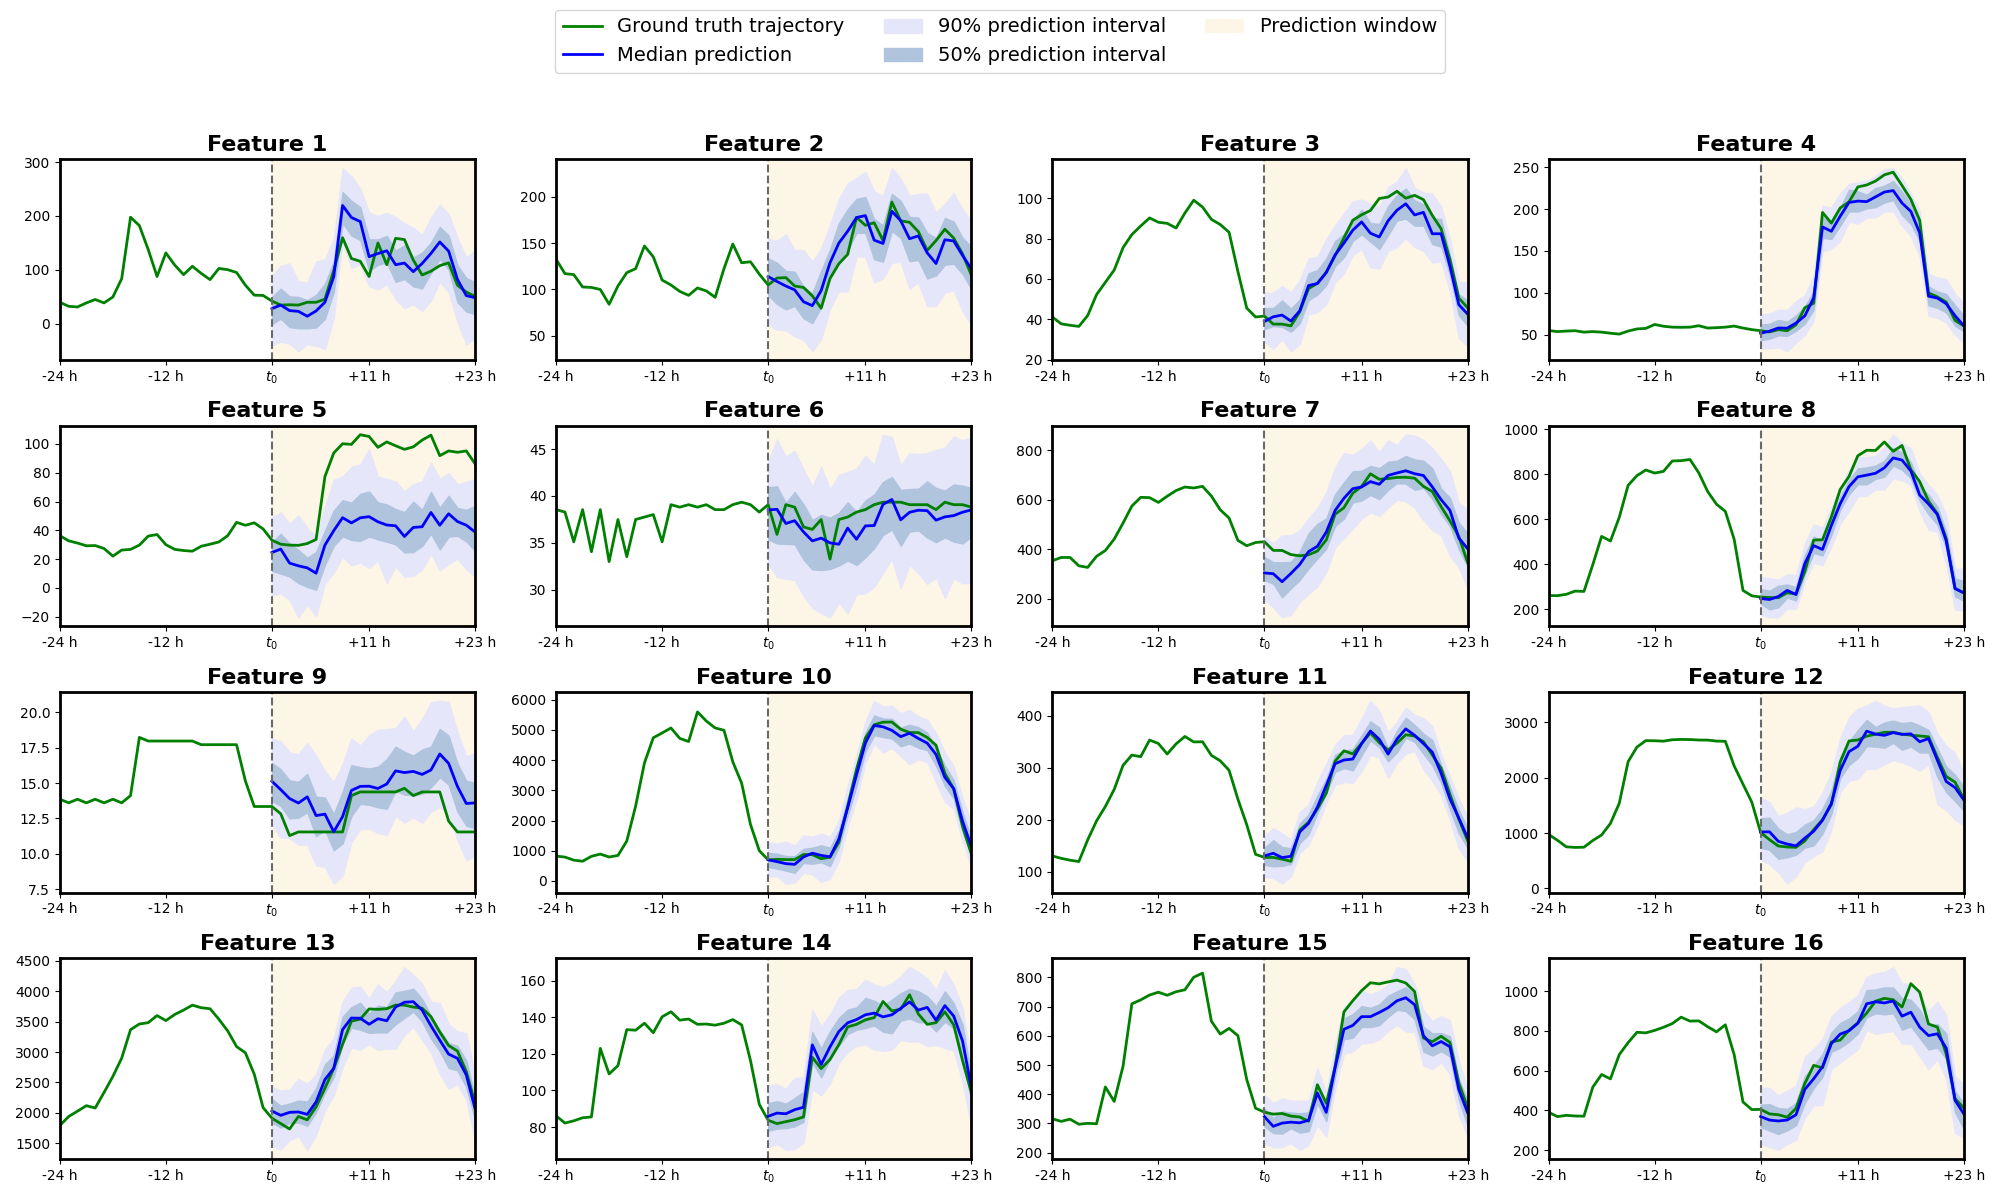
\includegraphics[width=\textwidth]{figures/ts_electricity.png}
    \caption{Prediction intervals of \algo{} for the first prediction window of the test set in the Electricity time series dataset. Only the first 16 features out of 370 are plotted.}
    \label{fig:ts_results}
\end{figure}
To illustrate \algo's new training objective does not degrade it as a generic sequence model, we evaluate \algo{} on high-dimensional and long-horizon sequence prediction tasks in time series prediction. We adopt multiple time series datasets with real-world applications from GluonTS~\cite{gluonts} and evaluate \algo{} with strong baselines with standard metrics in this domain. In this section, we mainly focus on the results and analysis. For a detailed description of datasets and the metric, we refer the reader to Appendix~\ref{app:dataset_timeseries}.

\paragraph{Problem Formulation}
Let $\boldsymbol{X} = \left\{ \mathbf{x}_t \right\}_{t=1}^T$ be a sequence (multivariate time series) of $D$-dimensional observations $\mathbf{x}_t \in \mathbb{R}^D$ of some underlying dynamical process, sampled in discrete time steps $t \in \left\{1, \dots, T\right\}$, where $T \in \mathbb{N}$. In the problem setting of probabilistic time series forecasting, the sequence $\boldsymbol{X} = \left\{ \boldsymbol{X}_c, \boldsymbol{X}_p \right\}$ is split into two subsequences at time step $t_0 \in \mathbb{N}$ with $1 < t_0 \leq T$: the context window $\boldsymbol{X}_c := \left\{ \mathbf{x}_t \right\}_{t=1}^{t_0-1}$ (also called history or evidence) of length $t_0-1$, and the prediction window $\boldsymbol{X}_p := \left\{ \mathbf{x}_t \right\}_{t=t_0}^{T}$ of length~$T - t_0 + 1$ (also known as the prediction horizon). Then, the task is to model the conditional joint probability distribution
\begin{equation} \label{eq:prediction_pdf}
    q{\left( \mathbf{x}_{t_0:T} \mid \mathbf{x}_{1:t_0-1} \right)} := \prod_{t=t_0}^T{q{\left( \mathbf{x}_t \mid \mathbf{x}_{1:t-1} \right)}}
\end{equation}
over the samples in the prediction window. If we know the distribution in~\eqref{eq:prediction_pdf}, we can sample forecast prediction sequences given some initial context from the evidence sequence. However, most time-dependent data generation processes in nature have complex dynamics and no tractable formulation of $q{\left( \mathbf{x}_{t_0:T} \mid \mathbf{x}_{1:t_0-1} \right)}$. Instead, we construct a statistical model that approximates the generative process in~\eqref{eq:prediction_pdf} and estimates quantiles via Monte Carlo sampling of simulated trajectories. In this way, confidence levels or uncertainty measures can be calculated, and point forecasts can be produced as the mean or median trajectory~\cite{hyndman2008forecasting}.

\paragraph{Results.}

\ctable[
    caption = {Results for time series forecasting. We report the test set $\text{CRPS}_\textbf{sum}$ (the lower, the better) of comparable methods on six time series datasets. We measure the mean and standard deviation of our method from five runs trained with different seeds.},
    label = {tab:results_ts},
    pos = ht,
    doinside = \scriptsize,
    center,
    star
]{lccccccc}{}{
    \FL
     Method & Exchange & Solar & Electricity & Traffic & Taxi & Wikipedia
    \ML
    VES~\cite{hyndman2008forecasting} & 0.005 $\pm$ 0.000 & 0.900 $\pm$ 0.003 & 0.880 $\pm$ 0.004 & 0.350 $\pm$ 0.002 & - & - \NN
    VAR~\cite{luetkepohl2007new} & 0.005 $\pm$ 0.000 & 0.830 $\pm$ 0.006 & 0.039 $\pm$ 0.001 & 0.290 $\pm$ 0.001 & - & - \NN
    VAR-Lasso~\cite{luetkepohl2007new} & 0.012 $\pm$ 0.000 & 0.510 $\pm$ 0.006 & 0.025 $\pm$ 0.000 & 0.150 $\pm$ 0.002 & - & 3.100 $\pm$ 0.004 \NN
    GARCH~\cite{weide2002garch} & 0.023 $\pm$ 0.000 & 0.880 $\pm$ 0.002 & 0.190 $\pm$ 0.001 & 0.370 $\pm$ 0.001 & - & - \NN
    DeepAR~\cite{salinas2020deepar} & - & 0.336 $\pm$ 0.014 & 0.023 $\pm$ 0.001 & 0.055 $\pm$ 0.003 & - & 0.127 $\pm$ 0.042 \NN
    LSTM-Copula~\cite{salinas2019highdimensional} & 0.007 $\pm$ 0.000 & 0.319 $\pm$ 0.011 & 0.064 $\pm$ 0.008 & 0.103 $\pm$ 0.006 & 0.326 $\pm$ 0.007 & 0.241 $\pm$ 0.033 \NN
    GP-Copula~\cite{salinas2019highdimensional} & 0.007 $\pm$ 0.000 & 0.337 $\pm$ 0.024 & 0.025 $\pm$ 0.002 & 0.078 $\pm$ 0.002 & 0.208 $\pm$ 0.183 & 0.086 $\pm$ 0.004 \NN
    KVAE~\cite{krishnan2016structured} & 0.014 $\pm$ 0.002 & 0.340 $\pm$ 0.025 & 0.051 $\pm$ 0.019 & 0.100 $\pm$ 0.005 & - & 0.095 $\pm$ 0.012 \NN
    NKF~\cite{bezenac2020normalizing} & - & 0.320 $\pm$ 0.020 & 0.016 $\pm$ 0.001 & 0.100 $\pm$ 0.002 & - & 0.071 $\pm$ 0.002 \NN
    Transformer-MAF~\cite{rasul2021multivariate} & 0.005 $\pm$ 0.003 & 0.301 $\pm$ 0.014 & 0.021 $\pm$ 0.000 & 0.056 $\pm$ 0.001 & 0.179 $\pm$ 0.002 & 0.063 $\pm$ 0.003 \NN
    TimeGrad~\cite{rasul2021autoregressive} & 0.006 $\pm$ 0.001 & 0.287 $\pm$ 0.020 & 0.021 $\pm$ 0.001 & {0.044} $\pm$ {0.006} & 0.114 $\pm$ 0.020 & 0.049 $\pm$ 0.002 \NN
    ScoreGrad sub-VP SDE~\cite{yan2021scoregrad} & 0.006 $\pm$ 0.001 & \textbf{0.256} $\pm$ \textbf{0.015} & \textbf{0.019} $\pm$ \textbf{0.001} & 0.041 $\pm$ 0.004 & {0.101} $\pm$ {0.004} & \textbf{0.043} $\pm$ \textbf{0.002} \NN
    \textbf{Ours} & \textbf{0.003} $\pm$ \textbf{0.001} & {0.289} $\pm$ {0.002} & {0.023} $\pm$ {0.001} & \textbf{0.040} $\pm$ \textbf{0.004} & \textbf{0.075} $\pm$ \textbf{0.002} & 0.085 $\pm$ 0.007
    \LL
}

We evaluate the effectiveness of \algo{} as a sequence model on the canonical task of multivariate time series forecasting by following the experiment setup of ~\cite{salinas2019highdimensional, rasul2021multivariate, rasul2021autoregressive, tang2021probabilistic, yan2021scoregrad}
Concretely, we benchmark \algo{} on the datasets Solar, Electricity, Traffic, Taxi, and Wikipedia. These datasets have different dimensionality, domains, and sampling frequencies, and capture seasonal patterns of different lengths. The features of each dataset are detailed in Table~\ref{tab:ts_data}. We access the datasets from GluonTS~\cite{gluonts}, and set the context and prediction windows to the same length for each dataset. Additionally, we employ the same covariates as~\cite{rasul2021autoregressive}.
We evaluate the performance of the model quantitatively by estimating the Summed Continuous Ranked Probability Score $\operatorname{CRPS}_\text{sum}$ via quantiles. As a metric, $\operatorname{CRPS}_\text{sum}$ measures how well a forecast distribution matches the ground truth distribution.  We provide detailed descriptions of the metric in Appendix~\ref{app:dataset_timeseries}.
We benchmark with other diffusion-based methods in time series forecastings, such as TimeGrad~\cite{rasul2021autoregressive} and the transformer-based Transformer-MAF~\cite{rasul2021multivariate}. In particular, the main baseline of interest, TimeGrad~\cite{rasul2021autoregressive}, is a next-token diffusion sequence model trained with teacher forcing.
We track the $\operatorname{CRPS}_\text{sum}$ metric on the validation set and use early stopping when the metric has not improved for 6 consecutive epochs, while all epochs are fixed to 100 batches across datasets. We then measure the $\operatorname{CRPS}_\text{sum}$ on the test set at the end of the training, which we report in Table~\ref{tab:results_ts}. We use the exact same architecture and hyperparameters for all time series datasets and experiments.
\algo{} outperforms all prior methods except for ~\cite{yan2021scoregrad} with which Diffusion Forcing is overall tied, except for the Wikipedia dataset, on which Diffusion Forcing takes fourth place. 
Note that time series is not the core application of \algo{}, and that we merely seek to demonstrate that the Diffusion Forcing objective is applicable to diverse domains with no apparent trade-off in performance over baseline objectives. 

\subsection{Additional results in compositional generation}
\label{app:exp_compositionality}
Since \algo{} models the joint distribution of any subset of a sequence, we can leverage this unique property to achieve compositional behavior - i.e., \algo{} can sample from the distribution of \emph{subsets} of the trajectory and compose these sub-trajectories into new trajectories. 

In particular, we show that we can also have flexible control over how compositional \algo{} is. As shown in \ref{fig:compositionality}, consider a dataset of trajectories on a 2D, square plane, where all trajectories start from one corner and end up in the opposite corner, forming a cross shape. When no compositional behavior is desired, one can let the models replicate the cross-shaped distribution by allowing full memory of the HMM model. 
When one desires compositional such as generating a V-shaped trajectory, which stitches two sub-trajectories together, one can let the model generate shorter plans with no-memory context using MPC. (Add figures).

\begin{figure}[h]
    \centering
    \begin{subfigure}[t]{.3\linewidth}
        \centering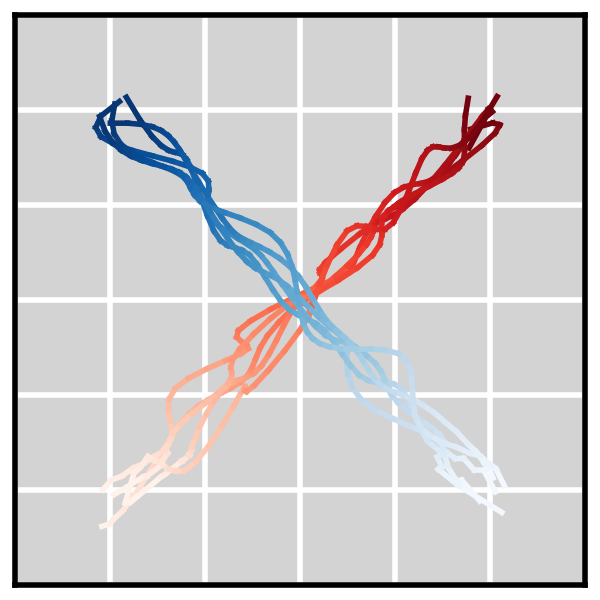
\includegraphics[width=\linewidth]{figures/dataset_diagonal2d_thick_v3.png}
        \caption{Dataset} \label{fig:compositionality_dataset}
    \end{subfigure}
    \begin{subfigure}[t]{.3\linewidth}
        \centering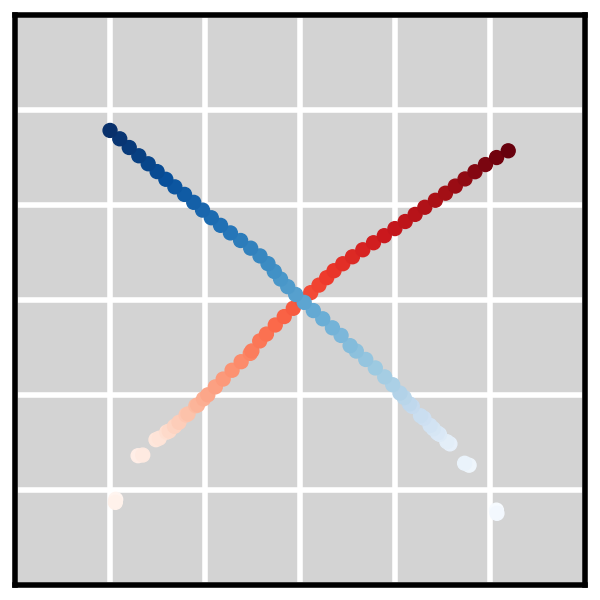
\includegraphics[width=\linewidth]{figures/w_memory.png}
        \caption{W/ memory} \label{fig:compositionality_w_memory}
    \end{subfigure}
    \begin{subfigure}[t]{.3\linewidth}
        \centering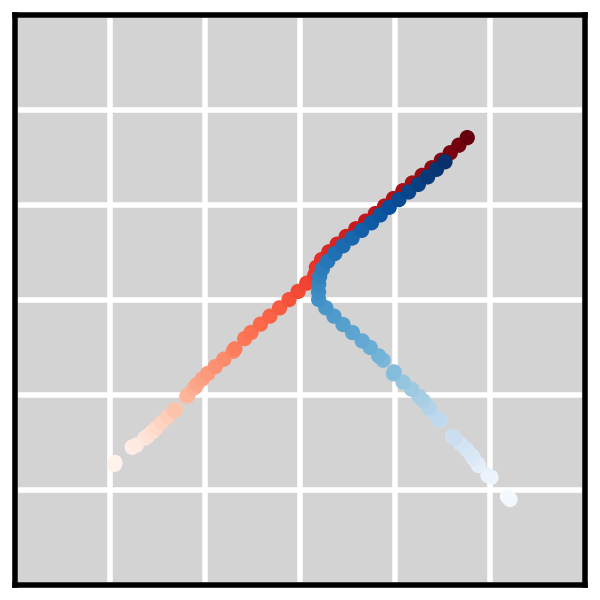
\includegraphics[width=\linewidth]{figures/wo_memory_v2.png}
        \caption{W/o memory} \label{fig:compositionality_wo_memory}
    \end{subfigure}
    \caption{Given a dataset of trajectories~(\subref{fig:compositionality_dataset}), \algo{} models the joint distribution of all subsequences of arbitrary length. At sampling time, we can sample from the trajectory distribution by sampling \algo{} with full horizon~(\subref{fig:compositionality_w_memory}) or recover Markovian dynamics by disregarding previous states~(\subref{fig:compositionality_wo_memory}).}
    \label{fig:compositionality}
\end{figure}



\subsection{Additional results in video prediction (wo/ cherry picking)}
\paragraph{Infinite Rollout without sliding window}
\algo{} can rollout longer than maximum training horizon\emph{without sliding window}. That is, we run \algo{}'s RNN continuously without ever reinitializing $\bz_0$. This is a surprising effect we observed from the rollout stabilization property of \algo{}. In Figure~\ref{fig:minecraft_long_0},~\ref{fig:dmlab_long_0}, we use \algo{} to generate video sequences of length $180$ and visualize subsampled sequences. Notably, \algo{} used in these visualizations is trained with a maximum length of $72$ frames for Minecraft and $36$ frames for DMLab, illustrating it can rollout 2x-5x times longer than it's trained on \emph{without sliding window}. In addition, we also tried rolling these models out for $2000$ frames and without seeing the model blowing up on both datasets. There are occasional cases where the Minecraft agent gets stuck and the entire screen is the ``dirt'' block, but this is more of a dataset issue~\ref{app:dataset_detail} and the agent is able to recover after it turns around. 

\begin{figure}[h]
    \centering
    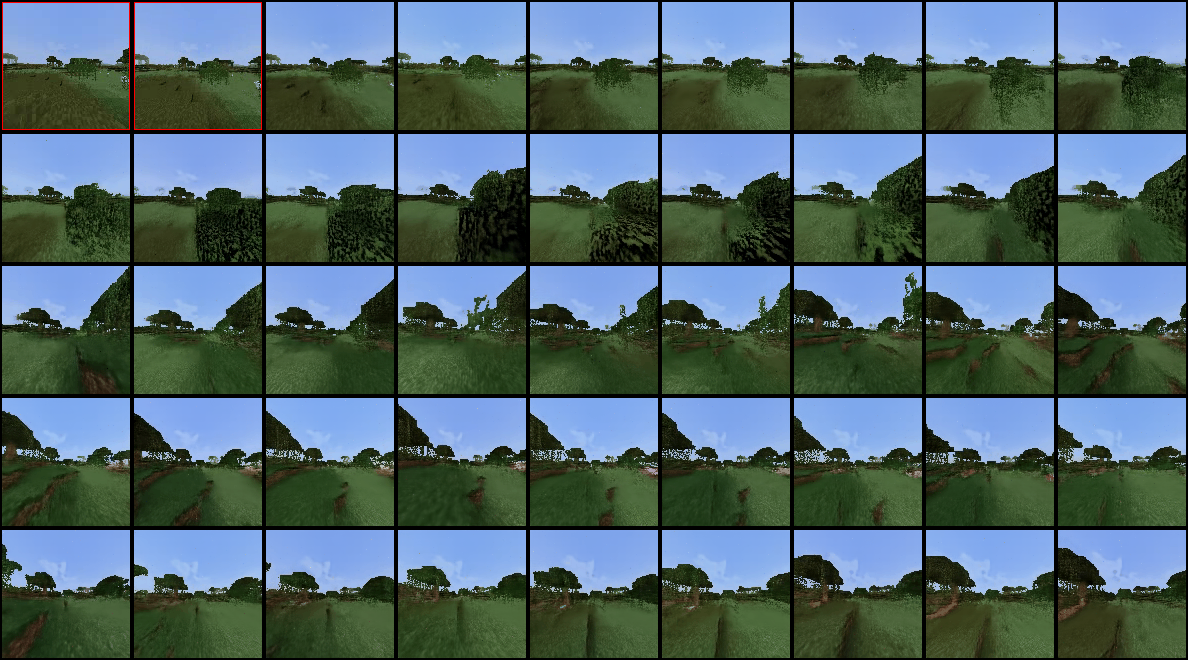
\includegraphics[width=\textwidth]{figures/appendix_vis/df_minecraft_long_1.png}
    \caption{Visualization shows \algo{} trained on $72$ frames is able to rollout $180$ frames on Minecraft dataset \emph{without sliding window}. The visualization shows a non-cherry-picked subsampling of these $180$ frames, although \algo{} can roll out much longer (such as 2000 frames) on this dataset.}
    \label{fig:minecraft_long_0}
\end{figure}
\begin{figure}[h]
    \centering
    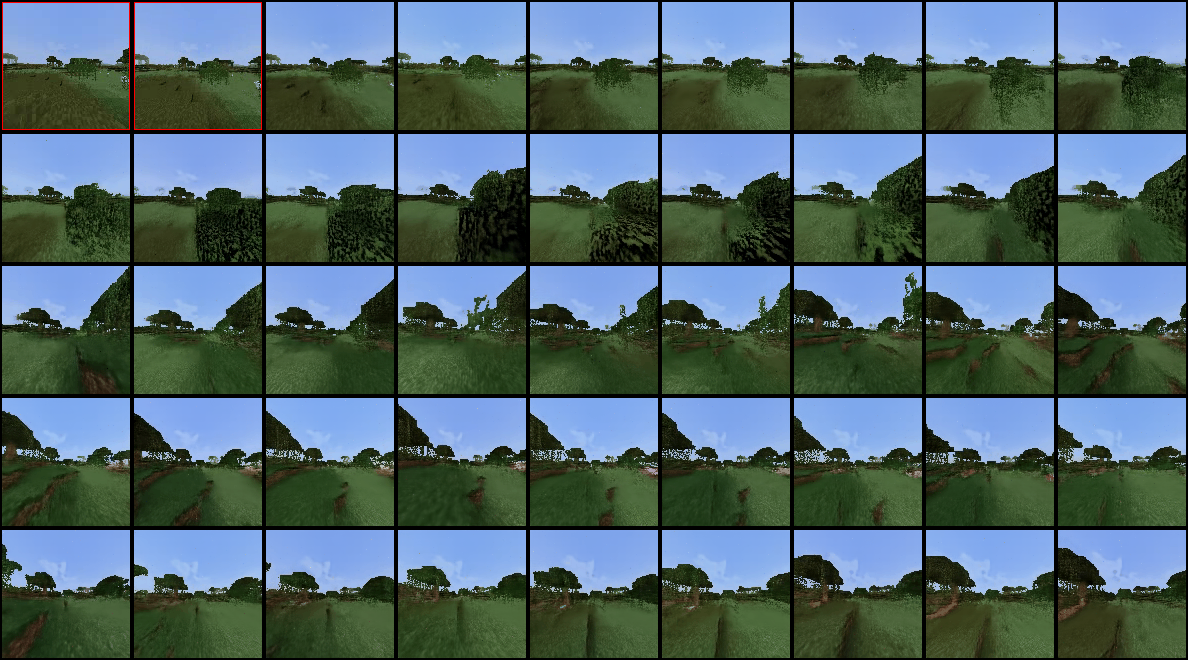
\includegraphics[width=\textwidth]{figures/appendix_vis/df_minecraft_long_1.png}
    \caption{\algo{} trained on $72$ frames is able to rollout $180$ frames on Minecraft dataset \emph{without sliding window}. The visualization shows a non-cherry-picked subsampling of these $180$ frames, although \algo{} can roll out much longer (such as 2000 frames) on this dataset. The first few frames marked in red are the ground truth images of the dataset used for conditioning.}
    \label{fig:minecraft_long_1}
\end{figure}
\begin{figure}[h]
    \centering
    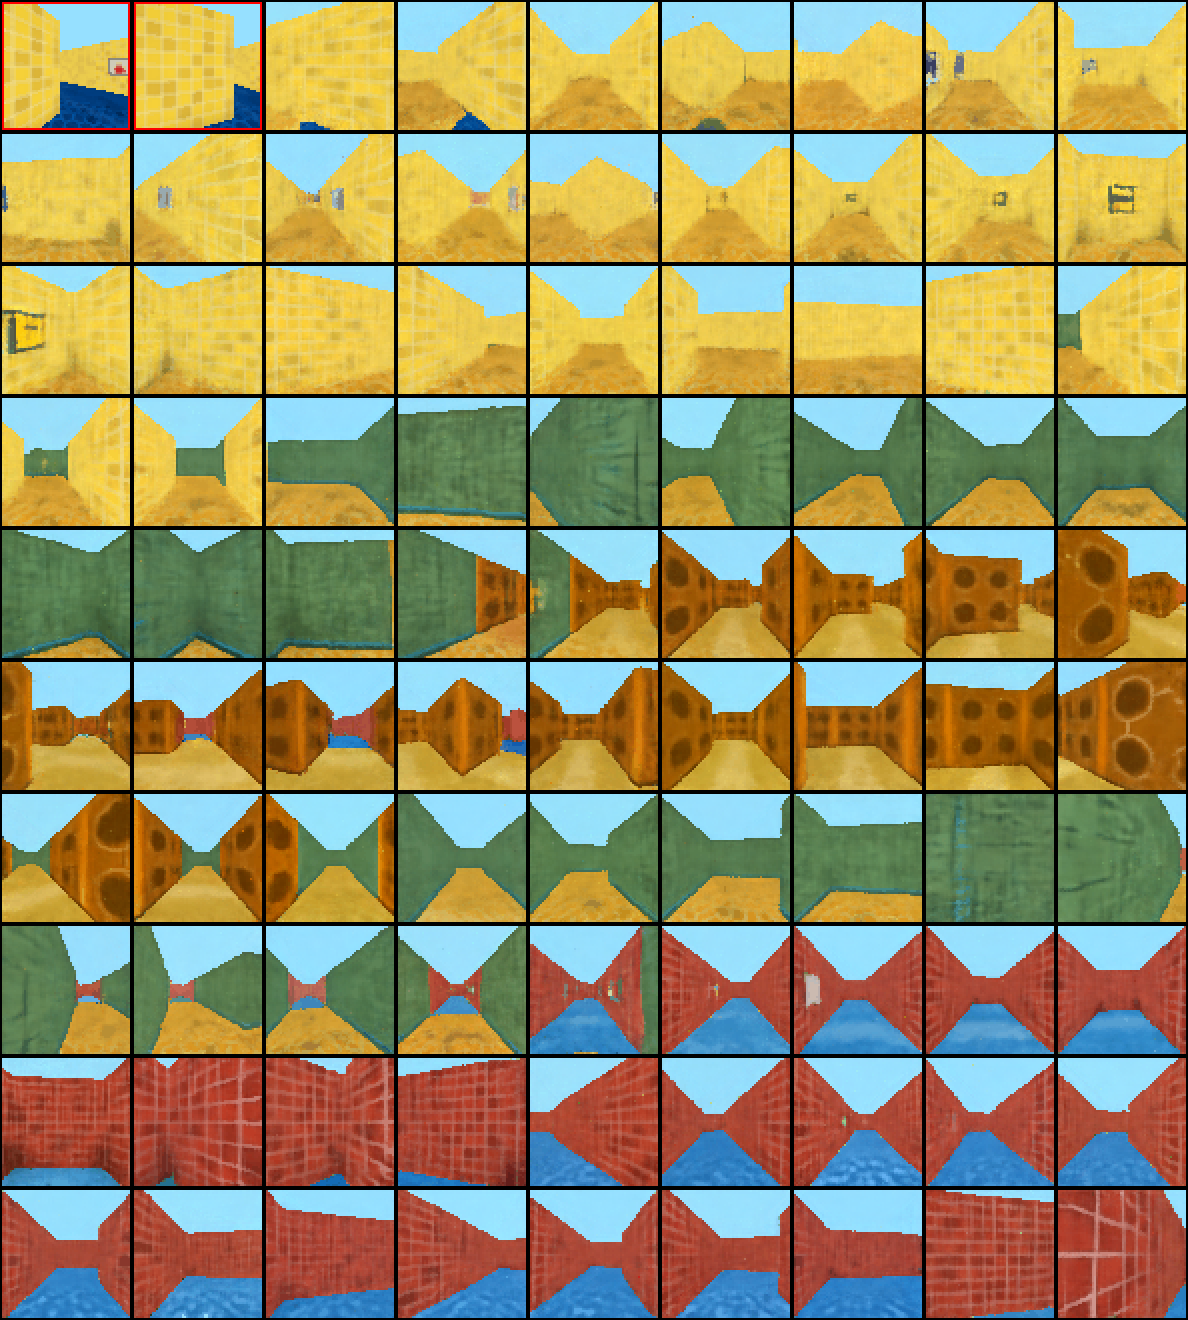
\includegraphics[width=\textwidth]{figures/appendix_vis/df_dmlab_long_0.png}
    \caption{Visualization shows \algo{} trained on $36$ frames is able to rollout $180$ frames on DMLab dataset \emph{without sliding window}. The visualization shows a non-cherry-picked subsampling of these $180$ frames, although \algo{} can roll out almost infinitely on this dataset. The first few frames marked in red are the ground truth images of the dataset used for conditioning.}
    \label{fig:dmlab_long_0}
\end{figure}
\begin{figure}[h]
    \centering
    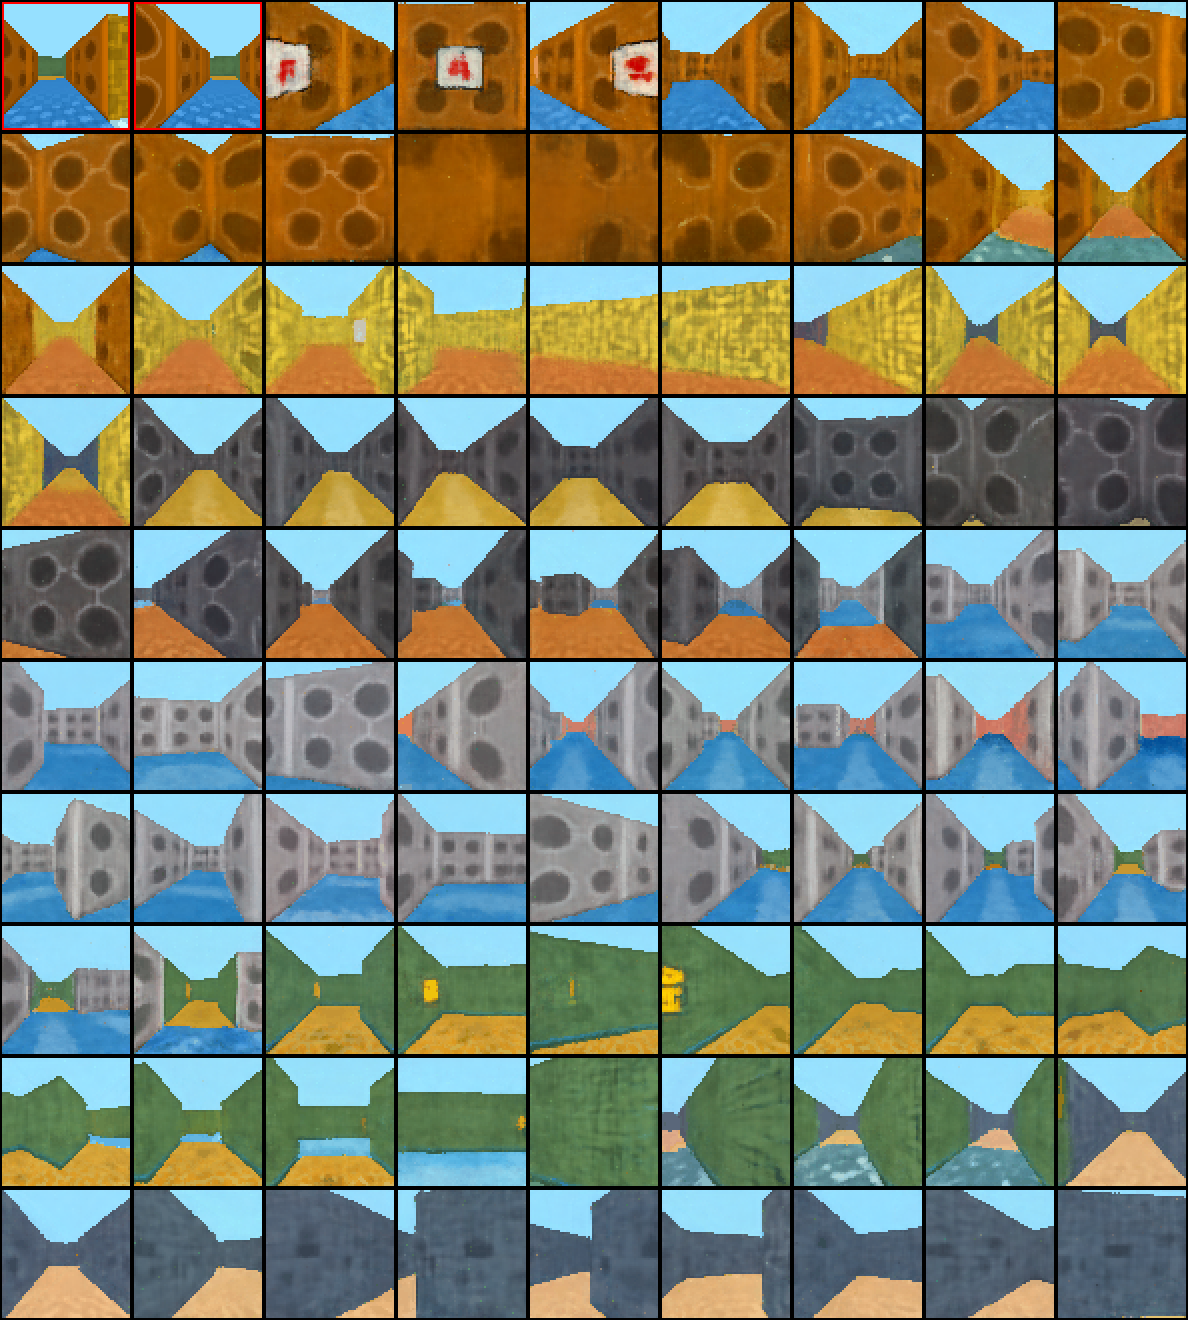
\includegraphics[width=\textwidth]{figures/appendix_vis/df_dmlab_long_1.png}
    \caption{Visualization shows \algo{} trained on $36$ frames is able to rollout $180$ frames on DMLab dataset \emph{without sliding window}. The visualization shows a non-cherry-picked subsampling of these $180$ frames, although \algo{} can roll out almost infinitely on this dataset. The first few frames marked in red are the ground truth images of the dataset used for conditioning.}
    \label{fig:dmlab_long_1}
\end{figure}

\paragraph{Consistency}
We also present additional results where we only generate within our maximum training length. As shown in figure~\ref{fig:minecraft_short}~\ref{fig:dmlab_short}, \algo{} can generate consistent videos. Results are not cherry-picked.
\begin{figure}[h]
    \centering
    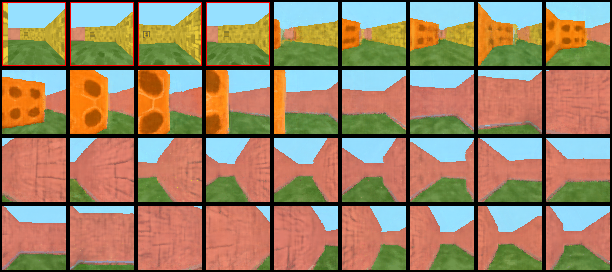
\includegraphics[width=\textwidth]{figures/appendix_vis/dmlab_df_0.png}
    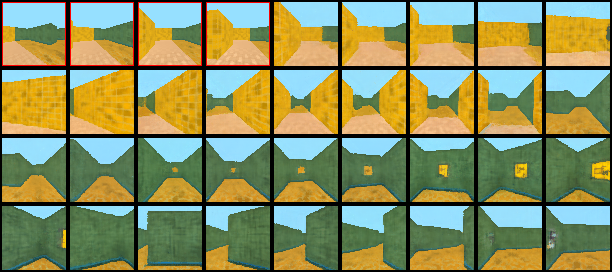
\includegraphics[width=\textwidth]{figures/appendix_vis/dmlab_df_1.png}
    \caption{Additional non-cherry-picked video prediction results on DMLab dataset, generated within maximum training length. The first few frames marked in red are the ground truth images of the dataset used for conditioning.}
    \label{fig:dmlab_short}
\end{figure}

\begin{figure}[h]
    \centering
    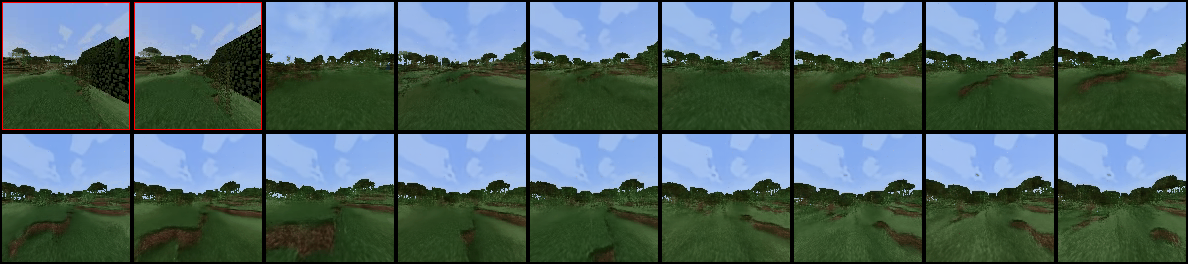
\includegraphics[width=\textwidth]{figures/appendix_vis/minecraft_df_0.png}
    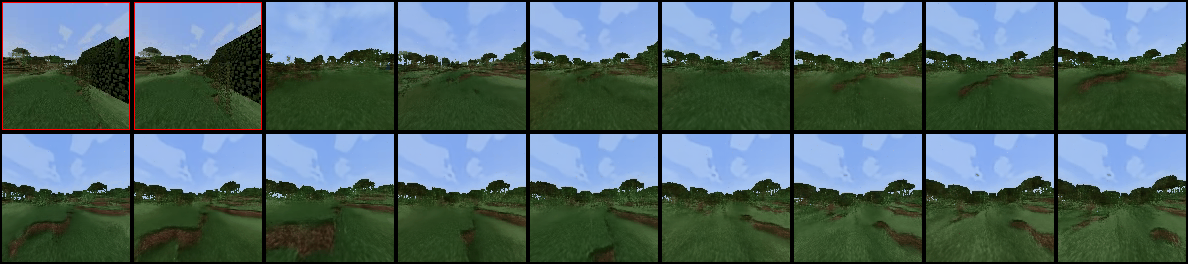
\includegraphics[width=\textwidth]{figures/appendix_vis/minecraft_df_0.png}
    \caption{Additional non-cherry-picked video prediction results on the Minecraft dataset, generated within maximum training length. The first few frames marked in red are the ground truth images of the dataset used for conditioning.}
    \label{fig:minecraft_short}
\end{figure}


\newpage

\subsection{Additional results in planning}
We provide some additional visualizations of causal planning in ~\ref{fig:df_plans_additional}. We also present additional visualization of \algo{} performing model predictive control in action. As shown in figure~\ref{fig:mpc_medium_0}, \algo{} can generate plans of shorter horizons since it's flexible horizon.
\begin{figure}[t]
    \centering
    \includegraphics[width=\textwidth]{figures/appendix_vis/df_medium_close_mpc.png}
    \caption{Example MPC planning for maze medium environment. Blue indicated trajectories actually executed already. Red is the plan.}
    \label{fig:mpc_medium_0}
\end{figure}

\begin{figure}[t]
    \centering
    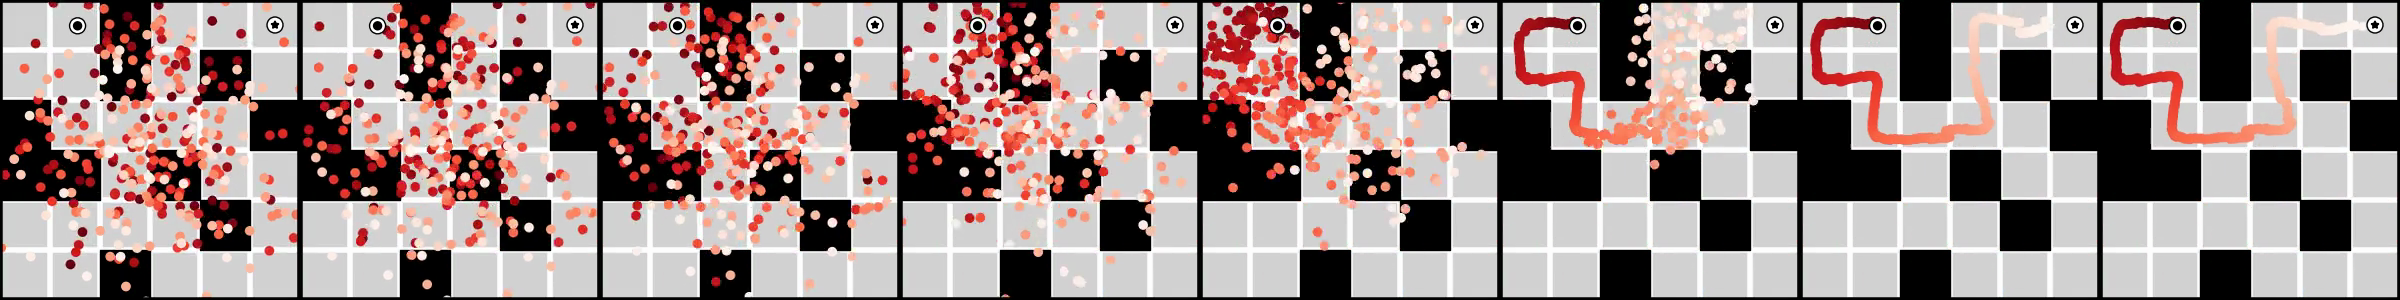
\includegraphics[width=\textwidth]{figures/appendix_vis/df_medium_close.png}
    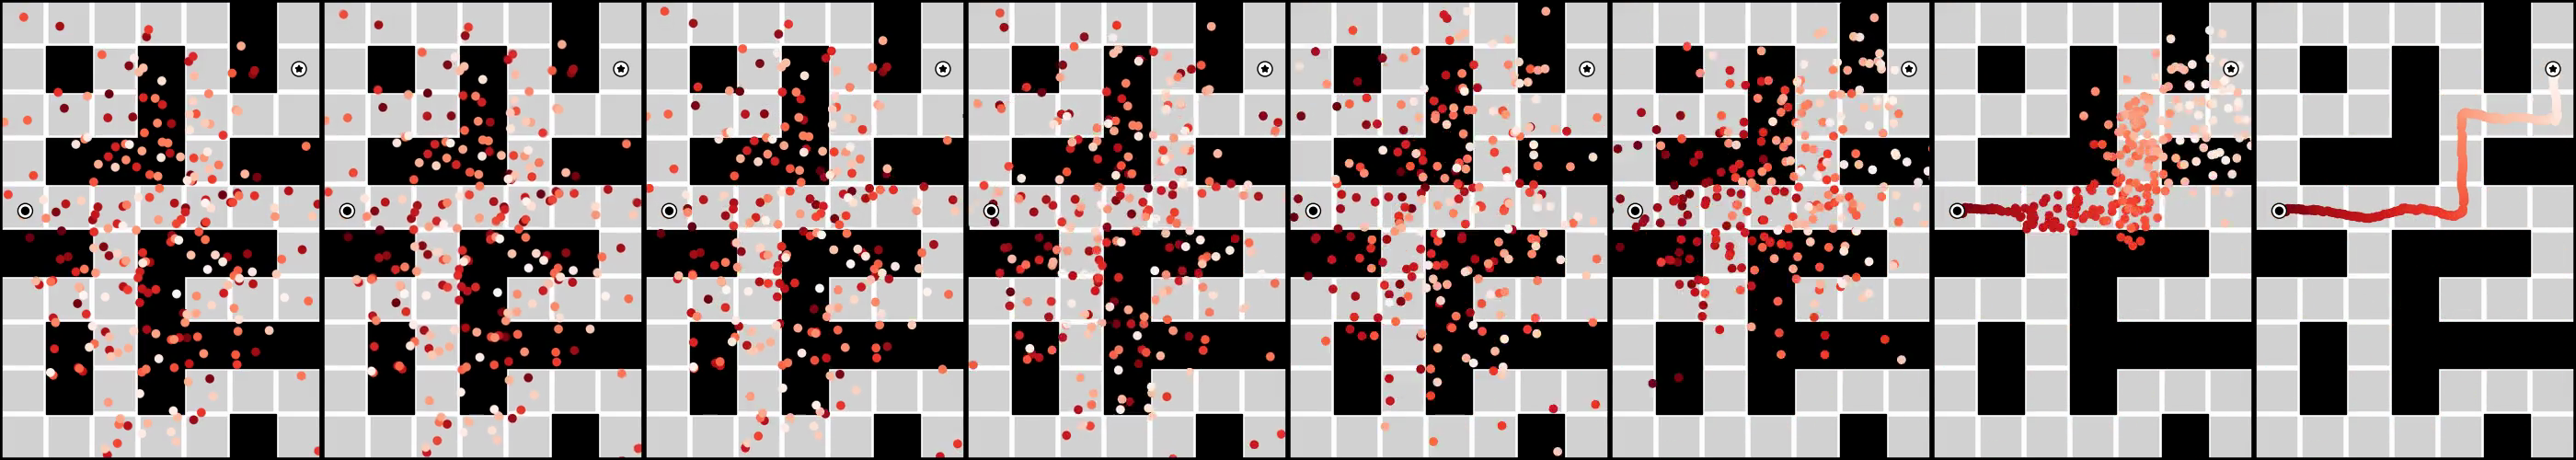
\includegraphics[width=\textwidth]{figures/appendix_vis/df_large_close.png}
    \caption{Example plans generated for maze medium (above) and maze large (below) environments.}
    \label{fig:df_plans_additional}
\end{figure}
\newpage

\subsection{Real robot experiment setup}
In Figure~\ref{fig:robot_currupted} we visualize our robot experiment setup with corruption on observation. The dataset is collected when the target bag isn't present, while we test with such a bag in the scene zero-shot for the imitation learning experiment with observation corruption. The typical failure mode is when the robot no longer reacts to the visual clues of the randomized location of objects. We didn't observe the robot act wildly due to visual distractors.

\begin{figure}[h]
    \centering
    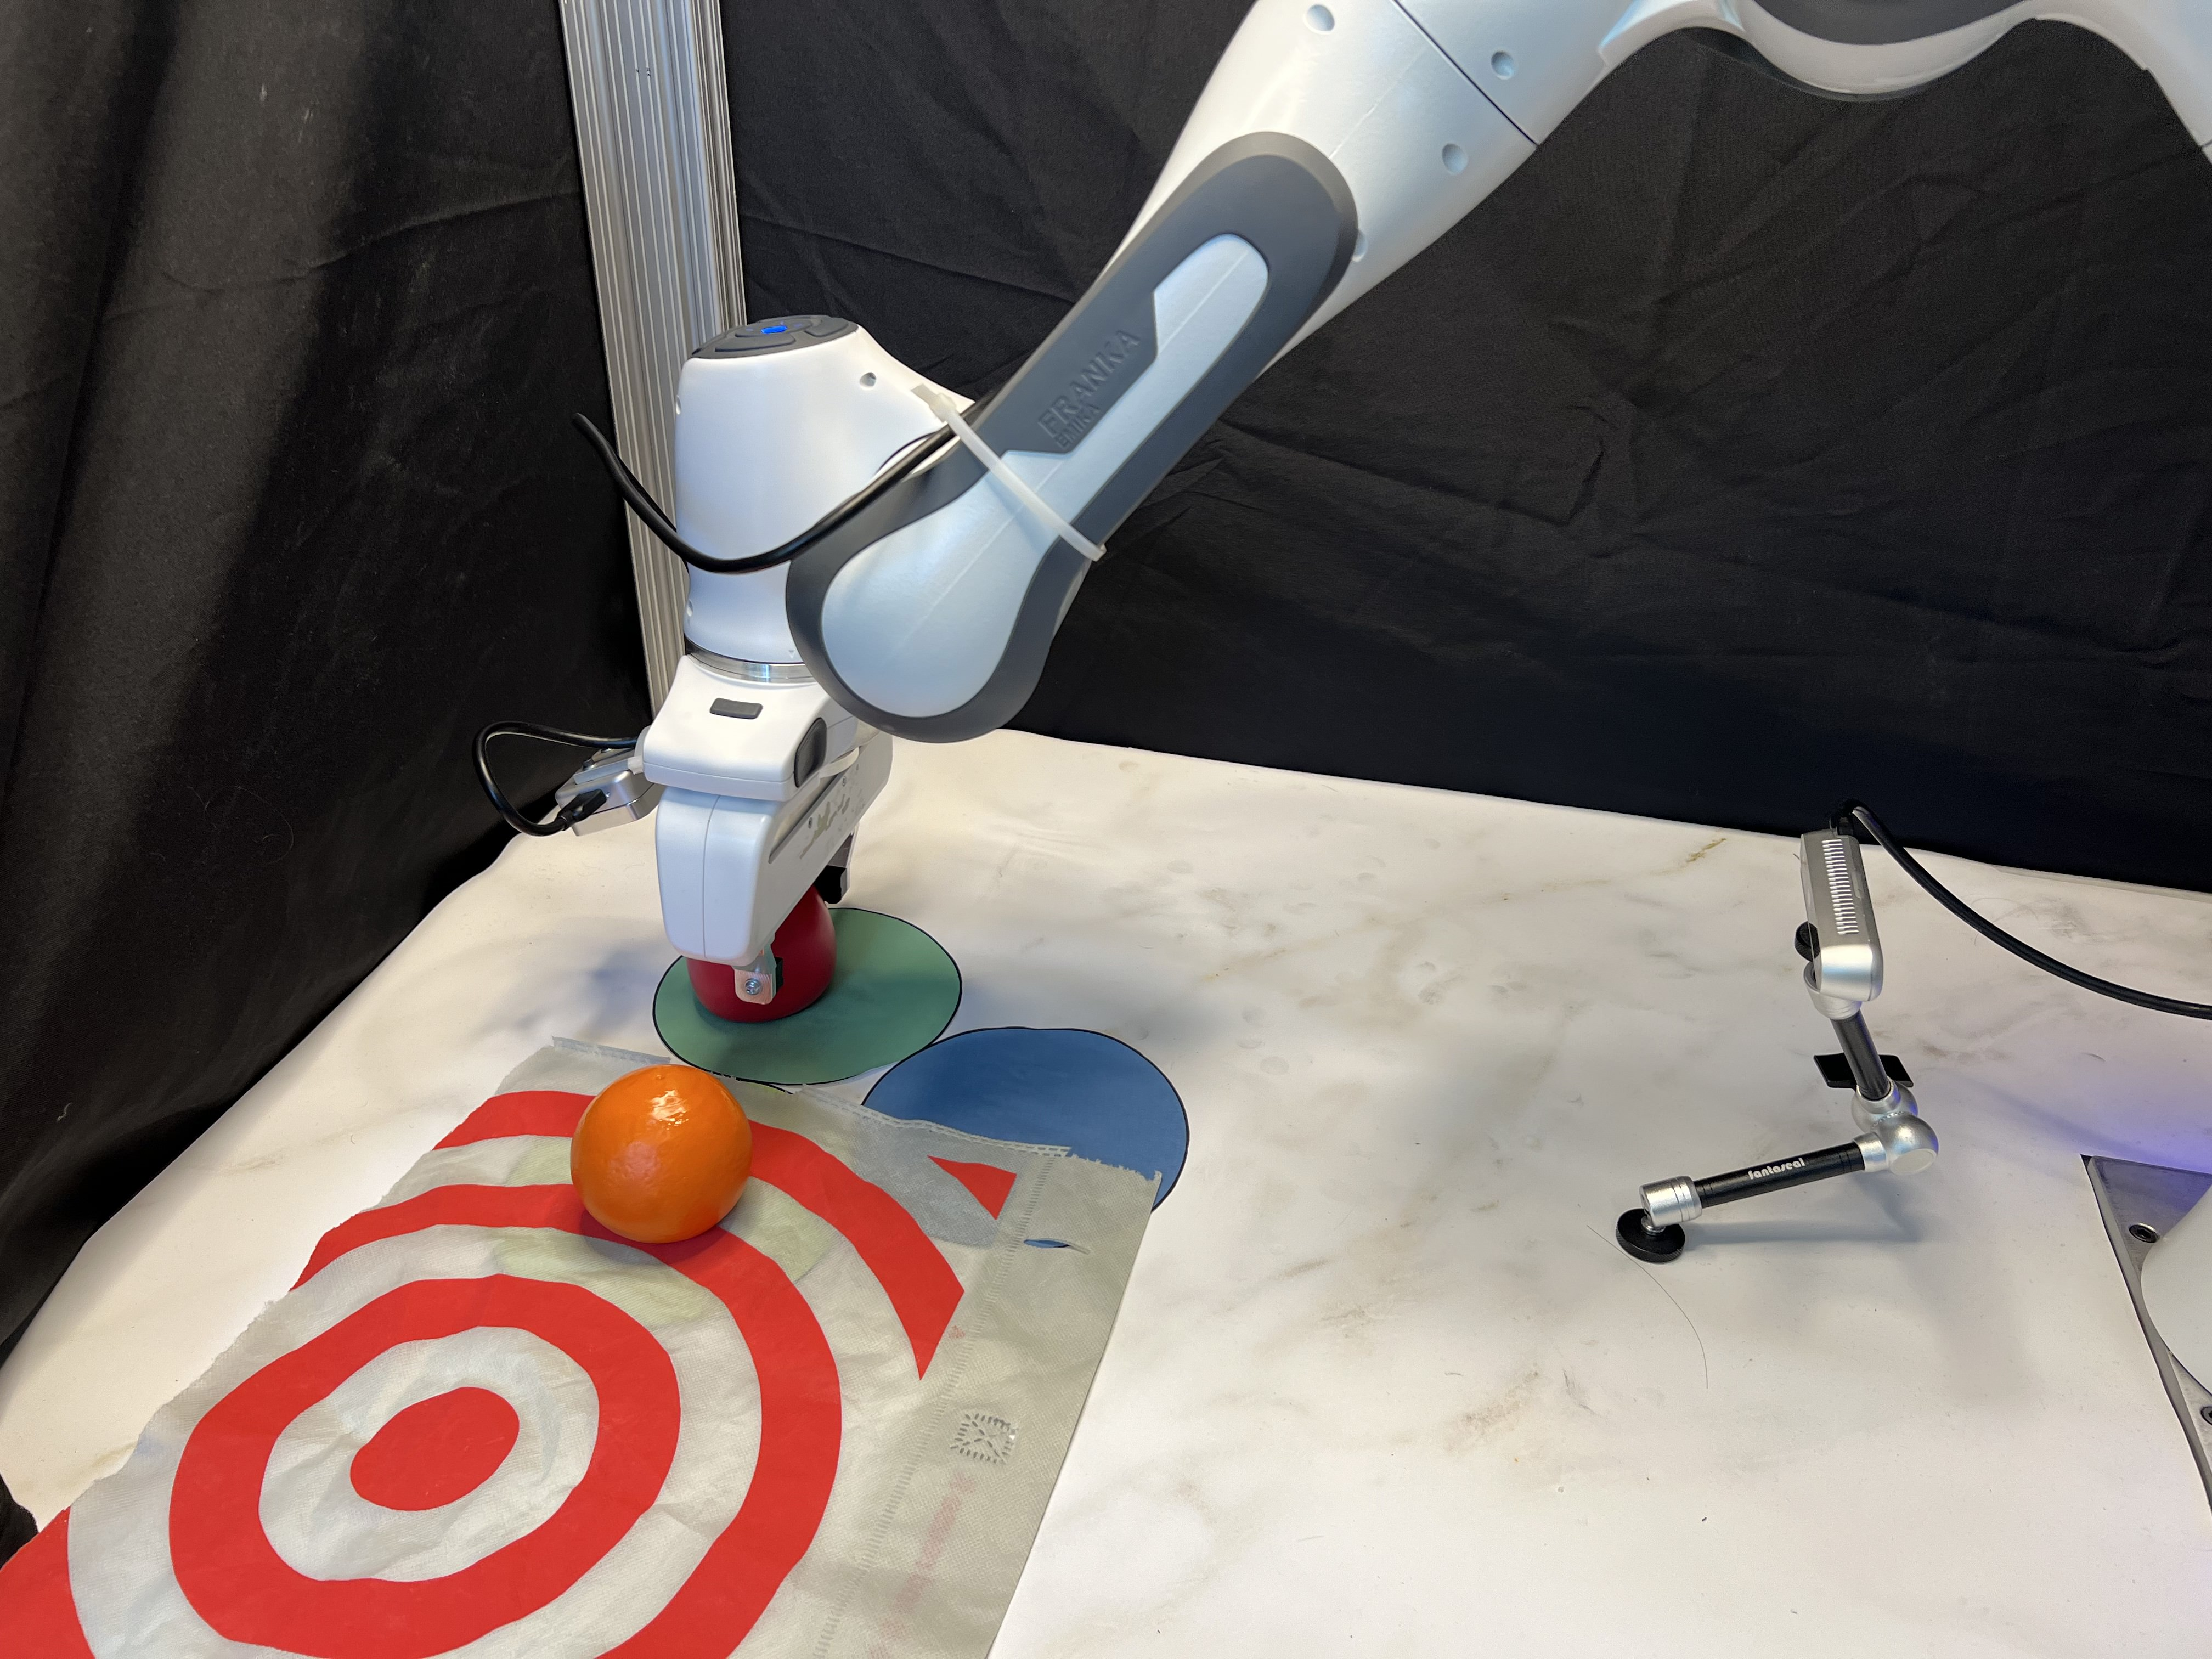
\includegraphics[width=0.5\textwidth]{figures/appendix_vis/robot_corrupt.jpg}
    \caption{We randomly throw a target bag on the table as a strong visual distractor. \algo{} can be prompted to treat observation as corrupted rather than ground truth.}
    \label{fig:robot_currupted}
\end{figure}
